\chapter{Theoretical Background}\label{chapter:background} \

In Chapter~\ref{chapter:background} we will introduce the
background information that is required to understand
the main ideas of this thesis. First we introduce
the basic concepts of quantum computing. Then we will
describe advanced concepts regarding quantum noise. We
assume some baseline \ac{ml} knowledge, however, we
will provide an outlook into \ac{qml}. Finally, we
present several types of adversarial machine learning
and adversarial training as a defense mechanism. \

\section{Fundamentals of Quantum Computing} \

First we introduce the qubit (Subsec.~\ref{subsection:qubit}),
the Bloch sphere (Subsec.~\ref{subsection:bloch}), and
multiple qubits (Subsec.~\ref{subsubsection:multiple_qubit}).
Afterwards, we present the operations to manipulate qubits in 
Subsection~\ref{subsection:gates}. Then, we describe entanglement
(Subsec.~\ref{subsubsection:entanglement}), a primordial
property of quantum mechanics. Thereafter, quantum circuits (Subsec.
~\ref{subsection:circuit}) and measurements (Subsec.
~\ref{subsection:measurement}) are explained. Finally, the
density operator (Subsec.~\ref{subsection:density_operator})
is defined to enable the description of noise in quantum systems. \

The information from this section is mainly based on Nielsen's
book~\cite{nielsen_quantum_2010}, further information regarding
quantum computing and quantum information can be found there. \

\subsection{Qubit}\label{subsection:qubit} \

The basic computing unit in quantum computing is the
\textit{qubit}~\cite{schumacher_quantum_1995}. Similar to the classical
bit, a qubit also has a state. While a bit has either a
\textit{0} or \textit{1} state, the qubit can have
many more states. The quantum equivalent to the classical
bit states would be \(\ket{0}\) and \(\ket{1}\) (spoken as \textit{ket}) in Dirac
notation~\cite{dirac_new_1939} and they represent the orthonormal computational
basis states in Equation~\ref{eq:qubit_bases}. \

\begin{equation}\label{eq:qubit_bases}
    \ket{0} = \begin{pmatrix}
                1 \\ 0
              \end{pmatrix} \qquad \qquad
    \ket{1} = \begin{pmatrix}
                0 \\ 1
              \end{pmatrix}
\end{equation} \

The complementing element to Dirac's notation is the \textit{bra}:
\(\bra{0}\) and \(\bra{1}\). The \textit{bra} is the conjugate transposed
vector from a \textit{ket}. The outer product of two vectors \(u\) and
\(v\) in dirac notation is written as \(\ketbra{u}{v}\). While the inner
product of the same vectors is expressed as \(\braket{u}{v}\). \

What makes the qubit different and more capable than
the classical bit is that it can also have different states
created by a linear combination or \textit{superposition} from
its basis states. The linear combination in Equation
~\ref{eq:qubit_superposition} is the complete representation
of a qubit, where \(\alpha\) and \(\beta\) are two complex numbers that
are denominated \textit{probability amplitudes}.
The values \(\alpha\) and \(\beta\) represent a distribution, in which
with probability \(|\alpha|^2\) we will observe a \textit{0}
value and with probability \(|\beta|^2\) we will observe a
\textit{1} value. This distribution is determined by the
Born rule~\cite{born_quantenmechanik_1926} and states that \(|\alpha|^2 + |\beta|^2 \stackrel{!}{=} 1\).
The Born rule thus implies that a qubit state is a unitary vector in
a two-dimensional complex vector space. Although the
probability amplitudes can take on any complex value as long
as they fulfill the Born rule, when we perform a measurement
in the computational base on the qubit it \textit{collapses}
to one of the two basis states. \

\begin{equation}\label{eq:qubit_superposition}
  \ket{\psi} = \alpha\ket{0} + \beta\ket{1}
\end{equation} \

In the real physical world qubits can be implemented by
several different mechanisms. However, the mathematical
qubit abstraction helps establish a baseline computing unit
for quantum computing independent of which mechanism it is
being represented by~\cite{nielsen_quantum_2010}. While in this perfect
mathematical description noise does not occur, there are
different mechanisms to represent the noise that quantum
computers suffer from, e.g. the density operator that will
be introduced in Subsection~\ref{subsection:density_operator}. \

\subsection{Bloch Sphere}\label{subsection:bloch} \

The qubit state from Equation~\ref{eq:qubit_superposition} can be
rewritten into Equation~\ref{eq:qubit_global_phase}, where \(e\)
is the Euler number, \(i\) is the imaginary number, and \(\gamma\),
\(\varphi\), and \(\theta\) are real numbers. \

\begin{equation}\label{eq:qubit_global_phase}
  \ket{\psi} = e^{i\gamma} \left( \cos{\frac{\theta}{2}}\ket{0} + e^{i\varphi}\sin{\frac{\theta}{2}}\beta\ket{1} \right)
\end{equation} \

Because for a single qubit the global phase \(e^{i\gamma}\) has no
observable effects, we can omit it and write the state of a qubit as: \

\begin{equation}\label{eq:qubit_bloch}
  \ket{\psi} = \cos{\frac{\theta}{2}}\ket{0} + e^{i\varphi}\sin{\frac{\theta}{2}}\beta\ket{1}
\end{equation} \

where \(\theta\) and \(\varphi\) determine a point in the Bloch
sphere~\cite{bloch_nuclear_1946}. The Bloch sphere (Fig.~\ref{fig:bloch_sphere})
is a helpful visual representation for understanding the state of a
qubit. In Section~\ref{section:noise} this representation will be
utilized to show the effects of quantum noise on a quantum state. It
can also be used to visualize the effect of the operations performed
on quantum states, these operations are called \textit{gates} and 
they will be introduced in Subsection~\ref{subsection:gates}. \

\begin{figure}[ht]
  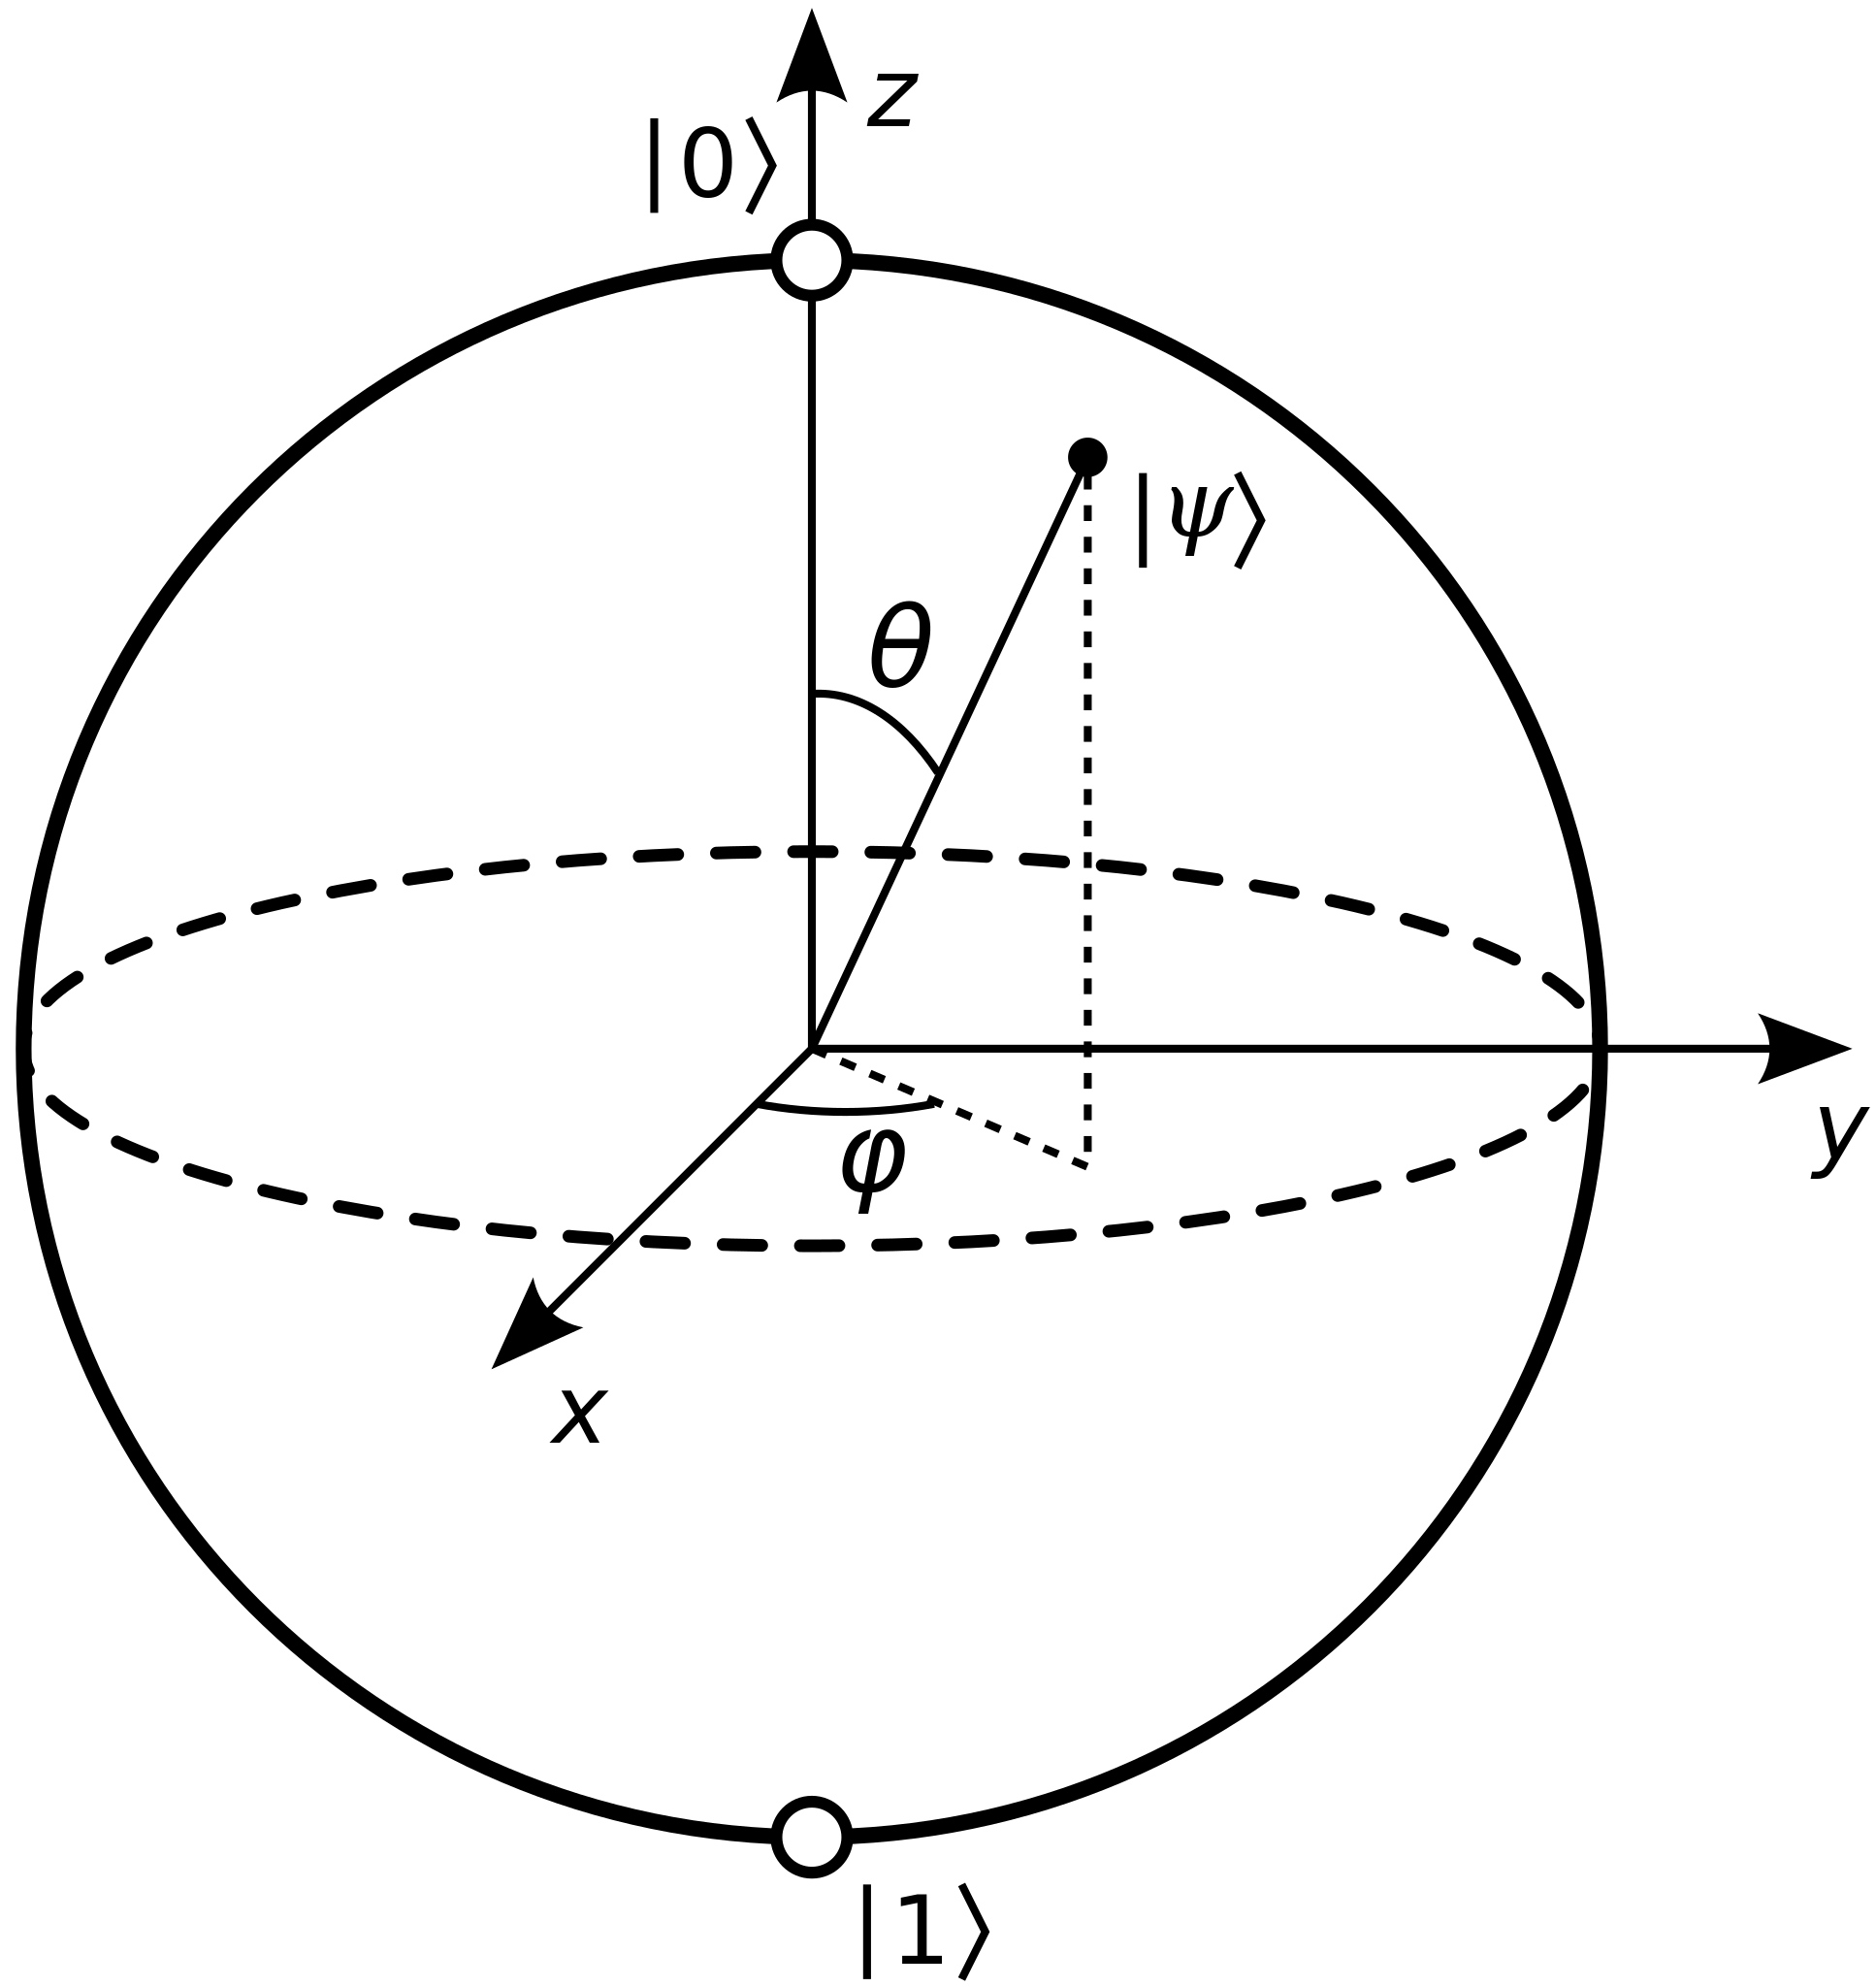
\includegraphics[scale=0.1]{figures/Bloch_sphere.png}
  \centering
  \caption{Bloch sphere representation of a qubit. Image taken from \href{https://commons.wikimedia.org/wiki/File:Bloch_Sphere.svg}{Wikimedia Commons} under the \href{https://en.wikipedia.org/wiki/Creative_Commons}{Creative Commons Attribution-Share Alike 3.0 Unported license}.}
~\label{fig:bloch_sphere}
\end{figure} \

\subsection{Multiple qubits} \

To describe multiple qubits we utilize the fundamentals presented in
Subsection~\ref{subsection:qubit} and expand them. For two qubits
\(\ket{00}, \ket{01}, \ket{10}\), and \(\ket{11}\) are the computational basis.
A general representation for a two qubit system can be found in 
Equation~\ref{eq:two_qubits}, where all the probability amplitudes must
follow the Born rule. \ 

\begin{equation}\label{eq:two_qubits}
  \ket{\psi} = \alpha_{00}\ket{00} + \alpha_{01}\ket{01} + \alpha_{10}\ket{10} + \alpha_{11}\ket{11}
\end{equation} \

Due to the Born rule the measurement results for
\(x = \left\{00, 01, 10, 11\right\}\) follow the probability
distribution determined by \(|\alpha_{x}|^2\). Similar to a
single qubit, once a measurement on both qubits is performed,
the state of the qubits will collapse to the measured
basis. Nevertheless, with multiple qubits we are able to perform
measurements on a subset of qubits. In the case of a two-qubit
system, measuring the first qubit will collapse its value. However,
the second's qubit state will remain. In the case of Eq.~\ref{eq:two_qubits},
if \textit{0} was measured in the first qubit, the amplitudes \(\alpha_{10}\)
and \(\alpha_{11}\) would disappear from the state as they are no longer
possible. Furthermore, the remaining amplitudes must be normalized,
such as in Eq.~\ref{eq:measure_first}, to fulfill the normalization
restriction.  \

\begin{equation}\label{eq:measure_first}
  \ket{\psi'} = \frac{\alpha_{00}\ket{00} + \alpha_{01}\ket{01}}
                    {\sqrt{|\alpha_{00}|^2 + |\alpha_{01}|^2}}
\end{equation} \

In Equation~\ref*{eq:multiple_qubits} we can find a general representation of
a set of \textit{n} qubits. For a system composed by \textit{n} qubits there are \(2^n\)
amplitudes. If we tried to simulate a quantum system with \(n = 50\), assuming
that complex numbers require 8 bytes to be stored~\cite{harris_array_2020}, a classical computer would need
approximately 9000 terabytes to store the generated quantum state. This simple calculation
shows the reason why quantum computers are so promising and also why classical computers
are not able to process quantum information efficiently. \
% (2**50)*8 = 9007199254740992
% https://docs.scipy.org/doc/numpy-1.17.0/user/basics.types.html

\begin{equation}\label{eq:multiple_qubits}
  \ket{\psi} = \alpha_{00}\ket{0\cdots0} + \cdots + \alpha_{2^{n-1}}\ket{1\cdots1}
\end{equation} \

\subsection{Quantum Gates}\label{subsection:gates}\

Once that quantum states have been defined, performing operations
on them is the next step to understand how quantum computing works.
These operations are denominated \textit{quantum gates} and they
modify the quantum state according to gates' properties. A quantum gate
can be represented as a matrix that fulfills one single property,
namely that it is a unitary matrix. In Equation~\ref{eq:unitary} we
can observe that a unitary matrix is one which when multiplied by its
own transpose conjugate is equal to the identity matrix.

\begin{equation}\label{eq:unitary}
  UU^{\dag} = I \qquad \qquad
  \ket{\psi} \xrightarrow{U} U\ket{\psi} = \ket{\psi'}
\end{equation}

This property is required because when a quantum gate is used on a
quantum state (Eq.~\ref{eq:unitary}), the resulting quantum state has to
be a valid normalized quantum state. By being a unitary matrix, this
effect is achieved. Applying a quantum gate to a quantum state can also be
mathematically interpreted as a matrix-vector multiplication between the
gate's unitary matrix and the quantum state vector. There are infinitely
many unitary matrices, however, there are some of specific importance.
The most important single-qubit quantum gates will be introduced in
Subsection~\ref{subsubsection:single_qubit}, while the most significant
multiple-qubits gates will be presented in 
Subsection~\ref{subsubsection:multiple_qubit} \

\subsubsection{Single-Qubit Gates}\label{subsubsection:single_qubit} \

Single-Qubit gates can be described by a two by two unitary matrix. The
first three quantum gates introduced are described by the Pauli matrices.
They are defined as the X, Y and Z gates because each matrix represents
a \(\pi\) rotation around the Bloch sphere in their respective axis. \

\paragraph{X Gate} \

The X gate's matrix and its gate representations can be found in
Equation~\ref{eq:pauli_x}. In classical computing, the X gate is
conceptually equivalent to the NOT gate, thus it
is also known as a quantum NOT gate. \

\begin{equation}\label{eq:pauli_x}
  X = \begin{pmatrix}
        0 & 1 \\
        1 & 0
      \end{pmatrix} \qquad \qquad
  \Qcircuit @C=1em @R=1em {
    & \gate{X} & \qw
  } \qquad
  \Qcircuit @C=1em @R=1em {
    & \targ & \qw
  }
\end{equation} \

In Equation~\ref{eq:pauli_x_basis} we can see the effect of the X
gate, where the computational basis states are flipped. This phenomena
is known as a \textit{bit flip}. \

\begin{equation}\label{eq:pauli_x_basis}
  X\ket{0} = \begin{pmatrix}
               0 & 1 \\
               1 & 0
             \end{pmatrix}
             \begin{pmatrix} 1 \\ 0 \end{pmatrix} = 
             \begin{pmatrix} 0 \\ 1 \end{pmatrix} =
             \ket{1}, \qquad
  X\ket{1} = \begin{pmatrix}
              0 & 1 \\
              1 & 0
            \end{pmatrix}
            \begin{pmatrix} 0 \\ 1 \end{pmatrix} = 
            \begin{pmatrix} 1 \\ 0 \end{pmatrix} =
            \ket{0}
\end{equation} \

\paragraph{Z Gate} \

Unlike the X gate, there is no conceptually equivalent
gate for the Z gate in classical computing. In Equation~\ref{eq:pauli_z}
we can observe the matrix and symbol representation of the Z gate. \

\begin{equation}\label{eq:pauli_z}
  Z = \begin{pmatrix}
        1 & 0 \\
        0 & -1
      \end{pmatrix} \qquad \qquad
  \Qcircuit @C=1em @R=1em {
    & \gate{Z} & \qw
  }
\end{equation} \

The effects of the Z gate can be found in Equation~\ref{eq:pauli_z_basis}.
We can observe that the \(\ket{0}\) state remains unmodified while
the \(\ket{1}\) state is negative after the operation. This phenomena
is known as a \textit{phase flip}. \

\begin{equation}\label{eq:pauli_z_basis}
  Z\ket{0} = \begin{pmatrix}
               1 & 0 \\
               0 & -1
             \end{pmatrix}
             \begin{pmatrix} 1 \\ 0 \end{pmatrix} = 
             \begin{pmatrix} 0 \\ 1 \end{pmatrix} =
             \ket{0}, \qquad
  Z\ket{1} = \begin{pmatrix}
               1 & 0 \\
               0 & -1
            \end{pmatrix}
            \begin{pmatrix} 0 \\ 1 \end{pmatrix} = 
            \begin{pmatrix} 1 \\ 0 \end{pmatrix} =
            -\ket{1}
\end{equation} \

\paragraph{Y Gate} \

The Y gate also doesn't have a conceptually equivalent gate
in classical computing. More interestingly the Y gate can be described
by the product of the X and Z matrix up to a global phase. The matrix
and symbol representation of the Y gate can be found in
Equation~\ref{eq:pauli_y}. \

\begin{equation}\label{eq:pauli_y}
  Y = \begin{pmatrix}
        0 & -i \\
        i & 0
      \end{pmatrix} \qquad \qquad
  \Qcircuit @C=1em @R=1em {
    & \gate{Y} & \qw
  }
\end{equation} \

In Equation~\ref{eq:pauli_y_basis} we can see how the Y gate
modifies the computational basis states. In it we can observe that
a bit flip and a phase flip have been executed, while \(i\) has been
added as a global phase. \

\begin{equation}\label{eq:pauli_y_basis}
  Y\ket{0} = \begin{pmatrix}
               0 & -i \\
               i & 0
             \end{pmatrix}
             \begin{pmatrix} 1 \\ 0 \end{pmatrix} = 
             \begin{pmatrix} 0 \\ 1 \end{pmatrix} =
             i\ket{1}, \qquad
  Y\ket{1} = \begin{pmatrix}
               0 & -i \\
               i & 0
            \end{pmatrix}
            \begin{pmatrix} 0 \\ 1 \end{pmatrix} = 
            \begin{pmatrix} 1 \\ 0 \end{pmatrix} =
            -i\ket{0}
\end{equation} \

As a complement to the Pauli gates, there are gates that
perform a specific \(\theta\) rotation around each axis of the
Bloch sphere. They are known as \(R_{X}\left(\theta\right)\),
\(R_{Y}\left(\theta\right)\) and \(R_{Z}\left(\theta\right)\).
Their unitary matrices and symbols can be found in Equation
~\ref{eq:rotation_gates}. \

\begin{equation}\label{eq:rotation_gates}
  \begin{split}
    R_X\left(\phi\right) = \begin{pmatrix}
          \cos\left(\frac{\phi}{2}\right) & -i\sin\left(\frac{\phi}{2}\right) \\
          -i\sin\left(\frac{\phi}{2}\right) & \cos\left(\frac{\phi}{2}\right)
        \end{pmatrix} \qquad \qquad \qquad
    R_Z\left(\phi\right) = \begin{pmatrix}
          e^{-i\frac{\phi}{2}} & 0 \\
          0 & e^{i\frac{\phi}{2}}
        \end{pmatrix} \\
    R_Y\left(\phi\right) = \begin{pmatrix}
          \cos\left(\frac{\phi}{2}\right) & -\sin\left(\frac{\phi}{2}\right) \\
          \sin\left(\frac{\phi}{2}\right) & \cos\left(\frac{\phi}{2}\right)
        \end{pmatrix} \qquad
    \Qcircuit @C=1em @R=1em {
      & \gate{R_{X}(\phi)} & \gate{R_{Y}(\phi)} & \gate{R_{Z}(\phi)} & \qw
    }
  \end{split}
\end{equation} \

More importantly, each Pauli matrix can be derived up to a
global phase from their respective rotational gate for a
given angle \(\theta = \pi\).

% MAYBE: Expand on the general rotation gate RZ RY RZ

\paragraph{Hadamard Gate} \

The Hadamard gate is one of the most useful single-qubit gates.
It will be later used in Subsection~\ref{subsubsection:entanglement}
to create \textit{entanglement} between two different qubits. \

\begin{equation}\label{eq:hadamard}
  H = \frac{1}{\sqrt{2}} 
      \begin{pmatrix}
        1 & 1 \\
        1 & -1
      \end{pmatrix} \qquad \qquad
  \Qcircuit @C=1em @R=1em {
    & \gate{H} & \qw
  }
\end{equation} \

The effects of the Hadamard gate can be observed in
Equation~\ref{eq:hadamard_basis}. The resulting states from applying
the Hadamard gate to the computational basis are denominated
\(\ket{+}\) and \(\ket{-}\) respectively and they represent
a superposition with equal probability for both computational 
basis to be measured. \

\begin{equation}\label{eq:hadamard_basis}
  H\ket{0} = \frac{1}{\sqrt{2}} \left( \ket{0} + \ket{1} \right) = \ket{+} \qquad
  H\ket{1} = \frac{1}{\sqrt{2}} \left( \ket{0} - \ket{1} \right) = \ket{-}
\end{equation} \

Another interesting property of the previously mentioned single-qubit
gates is that all of them are involutory. An involutory matrix is a
square matrix that is its own inverse. This implies that performing
twice the same gate will not modify the quantum state as the identity
transformation would have been applied. \

% MAYBE: Add S and T gates

\subsubsection{Multiple-Qubits Gates}\label{subsubsection:multiple_qubit} \

Multiple-Qubits gates are not that different from single-qubit gates,
they still have to be unitary. Nevertheless, depending on the qubits
that the gate is trying to modify, the size of the matrix will change.
Formally, if a gate is applying a transformation to \(n\) qubits, then
the dimensions of the gate's matrix \(M \in \mathbb{C}^{2^n \times 2^n}\).
Therefore, if \(n = 2\) then \(M\) would have the size
\(\mathbb{C}^{4 \times 4}\). \

\paragraph{Controlled NOT Gate} \

The~\ac{cnot} gate is a two-qubit quantum gate. It has a
\textit{control} qubit and a \textit{target} qubit. In
Equation~\ref{eq:cnot} we can observe the matrix and
symbol representation where the first qubit is the control
qubit and the second is the target qubit. \

\begin{equation}\label{eq:cnot}
  CNOT = \begin{pmatrix}
          1 & 0 & 0 & 0 \\
          0 & 1 & 0 & 0 \\
          0 & 0 & 0 & 1 \\
          0 & 0 & 1 & 0 \\
        \end{pmatrix} \qquad \qquad
  \Qcircuit @C=1em @R=1em {
      & \ctrl{1} & \qw \\
      & \targ & \qw \\
  } \qquad \qquad
  \begin{matrix}
    CNOT\ket{00} = \ket{00} \\
    CNOT\ket{01} = \ket{01} \\
    CNOT\ket{10} = \ket{11} \\
    CNOT\ket{11} = \ket{10} \\
  \end{matrix}
\end{equation} \

The effects of the \ac{cnot} gate can be seen in Equation~\ref{eq:cnot},
where depending on the value of the control qubit, a NOT gate will be
applied on the target wire. This can also be represented as
\(\ket{A,B}\rightarrow\ket{A,B\oplus A}\) performing an XOR between
the control and target qubits and storing the value in the second qubit. \

Regarding the~\ac{cnot} matrix in Equation~\ref{eq:cnot}, an intuiton
can be gained regarding the columns of the matrix, the computational
basis, and the effects of the gate. The ordering of the columns each
represent the input state with regards to the computational basis.
The first column represents \(\ket{00}\), the second column \(\ket{01}\),
the third column \(\ket{10}\) and so on. Moreover, the values that the vectors
represent in each column are associated with the output values after the gate
has been applied, e.g. \(\begin{pmatrix}1&0&0&0\end{pmatrix}^\top= \ket{00}\),
\(\begin{pmatrix}0&1&0&0\end{pmatrix}^\top= \ket{01}\),
\(\begin{pmatrix}0&0&1&0\end{pmatrix}^\top= \ket{10}\), etc. \

We can observe this phenomena between the third and fourth column in
Eq.~\ref{eq:cnot}, where the columns and values swap. Also this
intuiton helps us construct the matrix from the~\ac{cnot} gate when the
control and the target qubits have been inverted. In  Equation~\ref{eq:cnot_inverted}
we construct the matrix from the effects the CNOT gate would have in
the different computation basis states. \

\begin{equation}\label{eq:cnot_inverted}
  \begin{matrix}
    CNOT\ket{00} = \ket{00} \\
    CNOT\ket{01} = \ket{11} \\
    CNOT\ket{10} = \ket{10} \\
    CNOT\ket{11} = \ket{01} \\
  \end{matrix} \qquad \qquad
  \Qcircuit @C=1em @R=1em {
      & \targ & \qw \\
      & \ctrl{-1} & \qw \\
  } \qquad \qquad
  CNOT_2 = \begin{pmatrix}
    1 & 0 & 0 & 0 \\
    0 & 0 & 0 & 1 \\
    0 & 0 & 1 & 0 \\
    0 & 1 & 0 & 0 \\
  \end{pmatrix}
\end{equation} \

\paragraph{SWAP gate} \

The SWAP gate's effect are introduced in Equation~\ref{eq:swap}. It shows
that the value of the first qubit is swapped with the value of the
second qubit. Therefore, the gate will only have an effect if the qubits'
values are different. \

\begin{equation}\label{eq:swap}
  SWAP = \begin{pmatrix}
          1 & 0 & 0 & 0 \\
          0 & 0 & 1 & 0 \\
          0 & 1 & 0 & 0 \\
          0 & 0 & 0 & 1 \\
        \end{pmatrix} \qquad \qquad
  \Qcircuit @C=1em @R=1em {
    & \qswap & \qw \\
    & \qswap \qwx & \qw \\
  } \qquad \qquad
  \begin{matrix}
    SWAP\ket{00} = \ket{00} \\
    SWAP\ket{01} = \ket{10} \\
    SWAP\ket{10} = \ket{01} \\
    SWAP\ket{11} = \ket{11} \\
  \end{matrix}
\end{equation} \

The introduced two-qubit gates are also involutory. Therefore, applying
them twice would not modify the original quantum state. \

% MAYBE: Add toffoli gate

\subsection{Entanglement}\label{subsubsection:entanglement}
One of quantum mechanics most important concepts is entanglement, it is
also what fundamentally enables quantum computing to potentially
perform better than classical computing. Entanglement occurs when
two or more particles' quantum states are correlated and cannot
be described or measured independently of each other. \

For two unentangled qubits with quantum states \(\ket{\phi}_A\)
and \(\ket{\psi}_B\) respectively, we can describe the composite
system formed by both qubits with the tensor product between their
quantum states (Eq.~\ref{eq:separable_states}). Quantum states
represented in this manner are referred to as separable states.
Entangled systems can't be represented as separable states. \

\begin{equation}\label{eq:separable_states}
  \ket{\Psi}_{AB} = \ket{\phi}_A \otimes \ket{\psi}_B
\end{equation} \

In quantum computing the simplest and most common sequence of
gates to entangle two qubits can be found in
Equation~\ref{eq:entanglement}, where the Hadamard gate puts
the first qubit in a superposition and the CNOT gate creates
a dependent relationship between both qubits. \

\begin{equation}\label{eq:entanglement}
  \Qcircuit @C=1em @R=1em {
    \lstick{\ket{0}} & \gate{H} & \ctrl{1} & \qw \\
    \lstick{\ket{0}} & \qw & \targ & \qw \\
  } \qquad \qquad
  \ket{\psi} = \frac{1}{\sqrt{2}} \left(\ket{00} + \ket{11}\right)
\end{equation}

Reminiscing the fact that measuring a qubit will collapse its quantum
state to one of the computational basis. In the case of \(\ket{\psi}\),
according to the effects of Equation~\ref{eq:measure_first}, measuring the
first qubit will eliminate one of the two possible states. If the measured
value of the first qubit is \textit{0}, then \(\ket{\psi'} = \ket{00}\).
If \textit{1} is measured, then \(\ket{\psi'} = \ket{11}\). In the case
where we measured \textit{0}, the second qubit will be \textit{0} when
it is measured, else the second qubit would be \textit{1}. Therefore,
without measuring the second qubit we can know the value it will take 
if it was measured. \

\begin{equation}\label{eq:bell_states}
  \begin{matrix}
    \ket{00} \implies \ket{\Phi^+} = \frac{1}{\sqrt{2}} \left(\ket{00} + \ket{11}\right) \\
    \ket{10} \implies \ket{\Phi^-} = \frac{1}{\sqrt{2}} \left(\ket{00} - \ket{11}\right) 
  \end{matrix} \qquad \qquad
  \begin{matrix}
    \ket{01} \implies \ket{\Psi^+} = \frac{1}{\sqrt{2}} \left(\ket{01} + \ket{10}\right) \\
    \ket{11} \implies \ket{\Psi^-} = \frac{1}{\sqrt{2}} \left(\ket{01} - \ket{10}\right)
  \end{matrix}
\end{equation} \

The quantum states created by the circuit in Equation~\ref{eq:entanglement}
with differring basis inputs are called Bell's states or EPR
states~\cite{einstein_can_1935}. The Bell's states represent the maximally entangled
state between two qubits. In Equation~\ref{eq:bell_states} we can observe
the four resulting states, where in the \(\Phi\) states the value of the
measured qubit will be the same as the non-measured qubit. For the \(\Psi\)
states, the value of the measured qubit will be the opposite of the
non-measured qubit. This relationship holds independent on whether the
first or the second qubit in the system is measured. \

Entanglement is one of the most powerful tools in quantum mechanics.
Some of the documented uses of entanglement (mainly using EPR states)
are superdense coding~\cite{bennett_communication_1992} and quantum
teleportation~\cite{bennett_teleporting_1993}. Quantum teleportation
describes transmitting quantum information from a sender to a receiver
in a different location by sending only classical data. Superdense
coding refers to transferring a certain amount of classical bits of
information using a lesser number of qubits, therefore, sending more
information with less resources. \

\subsection{Quantum Measurement}\label{subsection:measurement} \

So far performing a measurement will collapse the quantum state to
one of the two computational basis. Nonetheless, a quantum state
can be measured in several different basis depending on the
measurement operator that is being used. Quantum measurements
are defined by a set \(M_m\) of measurement operators. This
set must fulfill the \textit{completeness equation} property
(Eq.~\ref{eq:completeness}) where all the operators must add
to the identity matrix. This property can be interpreted as
all the probability amplitudes from the quantum state must
add up to one. \

\begin{equation}\label{eq:completeness}
    \sum_{m}M_m^{\dag}M_m = I 
    \implies \sum_{m}p\left(m\right) = \sum_{m}\bra{\psi}M_m^{\dag}M_m\ket{\psi} = 1
\end{equation} \

Given a quantum state \(\ket{\psi}\) right before a measurement, the
probability of measuring \(m\) is defined as
\(p\left(m\right) = \bra{\psi}M_m^{\dag}M_m\ket{\psi}\).
The quantum state after the measurement \(\ket{\psi'}\) is described in
Equation~\ref{eq:state_after}. \

\begin{equation}\label{eq:state_after}
  \ket{\psi'} = \frac{M_m\ket{\psi}}{\sqrt{\bra{\psi}|M_m^{\dag}M_m|\ket{\psi}}}
\end{equation}

We can apply this framework to the computational basis. The
measurement operators of the computational basis are
\(M_0 = \ketbra{0}{0}\) and \(M_1 = \ketbra{1}{1}\). Both
of the operators are Hermitian, thus they are equal to their
conjugate transpose and \(M_m^{\dag}M_m = M_m^2\). 
Solving the square matrix of both measurement operators 
yields the original matrix \(M_m^2 = M_m\). We can observe
now that the completeness property is fulfilled in
Equation~\ref{eq:completeness_computational}. \

\begin{equation}\label{eq:completeness_computational}
  M_0^{\dag}M_0 + M_1^{\dag}M_1 = M_0 + M_1 = I
\end{equation} \

For a state \(\ket{\psi} = \alpha\ket{0} + \beta\ket{1}\) we
can utilize this new framework to explain what the probability
of measuring \textit{0} or \textit{1} is. In Equation~\ref{eq:probability}
we can observe that the probability of measuring \textit{0} is
\(\abs{\alpha}^2\), equal to the magnitude mentioned
in Subsection~\ref{subsection:qubit}. \

\begin{equation}\label{eq:probability}
  p\left(0\right) = \bra{\psi}M_0^{\dag}M_0\ket{\psi} =
  \bra{\psi}M_0\ket{\psi} = \abs{\alpha}^2
\end{equation} \

With Equation~\ref{eq:probability} we can also easily derive that the probability for
measuring the value \textit{1} is \(p\left(1\right) = \abs{\beta}^2\).
In Equation~\ref{eq:state_after_computational} we calculate how measuring
affects the quantum state, we use Equation~\ref{eq:state_after} with the
derived probability values. Recalling that a global phase has no effect
in a qubit (Subsection~\ref{subsection:bloch}), we can assume that
\(\frac{\alpha}{\abs{\alpha}}\ket{0} = \ket{0}\) and
\(\frac{\beta}{\abs{\beta}}\ket{1} = \ket{1}\). \

\begin{equation}\label{eq:state_after_computational}
    \ket{\psi_0'} = \frac{M_0\ket{\psi}}{\abs{\alpha}} =
    \frac{\alpha}{\abs{\alpha}}\ket{0} \qquad \qquad
    \ket{\psi_1'} = \frac{M_1\ket{\psi}}{\abs{\beta}} =
    \frac{\beta}{\abs{\beta}}\ket{1}
\end{equation} \

One would assume that knowing the magnitude of the probability amplitudes
is enough to reconstruct a quantum state, however, this is not the case.
For the states \(\ket{+}\) and \(\ket{-}\) the probability of measuring
the value \textit{0} is \(p\left(0\right) = \frac{1}{2}\) and the probability
of measuring the value \textit{1} is \(p\left(1\right) = \frac{1}{2}\).
Nevertheless, the quantum states \(\ket{+}\) and \(\ket{-}\) are not
equivalent. This occurs because there isn't any quantum measurement capable
of discerning between quantum states unless they are orthonormal.\

To be able to differentiate \(\ket{+}\) and \(\ket{-}\) we
need to measure in a different basis composed by orthonormal vectors.
The normalization property assures that they will be valid quantum states.
The orthogonality property guarantees linear independence between vectors,
thus, they can describe any quantum state in terms of the basis. In
this case we can use \(\ket{+}\) and \(\ket{-}\) as the new vectors for
the basis. We ensure that the vectors are normalized by calculating the
inner product of the vectors with themselves \(\braket{+}{+}=\braket{-}{-}=1\).
We guarantee that the vectors are orthogonal by calculating the
inner product of the vectors with each other \(\braket{+}{-}=\braket{-}{+}=0\). \

\begin{equation}\label{eq:projector_hadamard}
  M_+ = \ketbra{+}{+} = \begin{pmatrix}
                          \frac{1}{2} & \frac{1}{2} \\
                          \frac{1}{2} & \frac{1}{2}
                        \end{pmatrix} \qquad \qquad
  M_- = \ketbra{-}{-} = \begin{pmatrix}
                          \frac{1}{2} & -\frac{1}{2} \\
                          -\frac{1}{2} & \frac{1}{2}
                        \end{pmatrix}
\end{equation} \

The measurement operators derived from the new basis can be found
in Equation~\ref{eq:projector_hadamard}. These operators can now
be used to calculate the probability to measure either \(\ket{+}\)
or \(\ket{-}\). Similar to the computational basis case, both
measurement projectors are Hermitian. Thus, we can derive the
expression for the probability to measure \(x \in \left\{+,-\right\}\)
where \(p\left(x\right) = \bra{\psi}M_x\ket{\psi}\). With this new
expression we can clearly differentiate in Equation~\ref{eq:hadamard_states}
the \(\ket{+}\) and \(\ket{-}\) quantum states. \

\begin{equation}\label{eq:hadamard_states}
  \begin{matrix}
    p\left(+\right) = \bra{+}M_+\ket{+} = 1 \\
    p\left(+\right) = \bra{-}M_+\ket{-} = 0
  \end{matrix} \qquad \qquad
  \begin{matrix}
    p\left(-\right) = \bra{+}M_-\ket{+} = 0\\
    p\left(-\right) = \bra{-}M_-\ket{-} = 1
  \end{matrix}
\end{equation} \

\subsubsection{Projective Measurement} \

Projective measurements are a special case of quantum measurements.
They are characterized by an \textit{observable}, denoted as \(M\),
which is a Hermitian operator acting on the state space of the observed system.
The observable's spectral decomposition is in Equation~\ref{eq:observable},
where we can see that \(M\) is composed by the sum of the projector \(P_m\)
multiplied by the corresponding eigenvalue \(m\). The observable's
eigenvectors form an orthonormal basis and its
eigenvalues are the possible values for the measurement. \

\begin{equation}\label{eq:observable}
  M = \sum_{m}mP_m
\end{equation} \

From the observable we can derive an expression in Equation~\ref{eq:expectation}
for the expectation value. This expression is often denoted as \(\ev{M}\).
The expectation value denotes the value of the average measurement with
respect to the observable. More importantly, the expectation value can be
interpreted as the weighted average of what would be measured over many experiments,
thus, analytically calculating the result of several trials. \ 

\begin{equation}\label{eq:expectation}
  \mathbb{E}\left(M\right) =
  \sum_{m}m*p\left(m\right) =
  \sum_{m}m\bra{\psi}P_m\ket{\psi} =
  \bra{\psi} \left(\sum_{m}mP_m\right) \ket{\psi} =
  \bra{\psi}M\ket{\psi}
\end{equation} \

The Pauli Z matrix is of special importance as an observable. In Equation
~\ref{eq:observable_z} we can find the spectral decomposition of the
Pauli Z matrix. It has the eigenvalues \textit{1} and \textit{-1}, that
correspond to its eigenstates \(\ket{0}\) and \(\ket{1}\). The eigenstates
match the computational basis and form its measurement operators. Hence,
the Pauli Z matrix is widely used as an observable for the computational
basis. \

\begin{equation}\label{eq:observable_z}
  Z = 1 * \ketbra{0}{0} + \left(-1\right) * \ketbra{1}{1}
\end{equation} \

% MAYBE: Standard Deviation / nielsen 88

% MAYBE: Talk about how to retrieve the probability amplitudes experimentally with statistics - schuld 105

\subsection{Quantum Circuit}\label{subsection:circuit} \

Quantum circuits have already been informally introduced (Eq.~\ref{eq:entanglement}),
however, formalizing their structure is essential to understand quantum computing.
The main components are the qubit (Subsec.~\ref{subsection:qubit}), quantum
gates (Subsec.~\ref{subsection:gates}), and quantum measurements (Subsec.~\ref{subsection:measurement}).
In Equation~\ref{eq:circuit} the qubits are represented as \textit{wires} and are
abstracted from their physical implementation. The quantum gates in the wire act
from left to right and there can be no loops. If there are any gates before a
control operation, the gates must be executed before, therefore, creating a
dependency between operations and wires. \

\begin{equation}\label{eq:circuit}
  \Qcircuit @C=1em @R=1em {
    \lstick{\ket{1}} & \gate{Y}         & \targ       & \meterB{Z} & \cw \\
    \lstick{}        & \multigate{2}{U} & \ctrlo{-1}  & \qw        & \qw \\
    \lstick{}        & \ghost{U}        & \qw         & \qw        & \qw \\
    \lstick{}        & \ghost{U}        & \qw         & \qw        & \qw
      \inputgroupv{2}{4}{1em}{1em}{\ket{\psi}}}
\end{equation} \

If there is no input state on the circuit's left side, the initial quantum
state is \(\ket{0}\). Otherwise, an initial quantum state affecting one
wire can be represented with a ket. Additionally, a multi-qubit initial
quantum state can be characterized by a ket containing the quantum state
and a curly brace referencing the affected wires. A unitary matrix \(U\)
acting as a quantum gate on several qubits can be represented as rectangle
that covers the modified wires. \

When using a control gate (e.g.~\ac{cnot}) the control wire is represented
with a black dot. A white dot can be used if the control value must be
\(\ket{0}\), which is equivalent to performing an X gate before and after
the value is controlled. Finally, the metronome symbol is utilized to indicate
a measurement of the qubit value in the wire it appears. An observable can be
specified, else, the measurement is performed with respect to the computational
basis. The result is an eigenvalue from the obersvable and becomes a
classical value, which is represented by using a double-lined wire. \

\subsection{Density Operator}\label{subsection:density_operator} \

The current definition of quantum states as amplitude state vectors is
enough to explain closed quantum systems. However, quantum computers
are open quantum systems, meaning that they are influenced by
their environment. This influence changes the notion from \textit{pure}
into \textit{mixed} quantum states. Mixed quantum states present a
probabilistic perspective of quantum states and are represented by the
density operator \(\rho\). The density operator is vital for the thesis,
as it is utilized to model noise in open quantum systems. \

The density operator describes a quantum system's state that is not
fully known. In Equation~\ref{eq:density_operator} we can find
the expression for the density operator, where the system is found
in the set of states \(\ket{\psi_i}\) with probability \(p_i\) where
\(i \in \left[1,N\right]\). \

\begin{equation}\label{eq:density_operator}
  \rho = \sum_{i=1}^{N}p_i\ketbra{\psi_i}{\psi_i}
\end{equation} \

The density operator is also called a density matrix and it has three main
properties. The first one is that all the density operators are Hermitian.
Secondly, the density matrix's trace must be equal to 1. Finally, all
density operators are positive semidefinite. Thus, for any quantum state
\(\ket{\psi}\) we have that \(\bra{\psi}\rho\ket{\psi} \geq 0\). For a
given density operator \(\rho\), we can quantify how pure the quantum
state is. The \textit{purity} \(\gamma\) of \(\rho\) is defined as 
\(\gamma\left(\rho\right) = \trace\left(\rho^2\right)\). For a pure state \(\rho\),
\(\gamma\left(\rho\right) = 1\), while for a mixed state the purity is less
than 1. The maximally mixed state is proportional to the identity matrix
and has a purity of \(1/d\), where \(d\) is the dimension of the Hilbert
space where \(\rho\) is defined. \

In Equation~\ref{eq:unitary} we showed how a unitary operation \(U\) modifies
the quantum state \(\ket{\psi}\). Given a state represented by the density
operator \(\rho\), in Equation~\ref{eq:density_evolution} we can observer the
effects of performing a unitary operation \(U\) to the state \(\ket{\psi'}\)
that appears with probability \(p_i\). \

\begin{equation}\label{eq:density_evolution}
  \rho \xrightarrow{U} \sum_{i=1}^{N}p_{i}U\ketbra{\psi_i}{\psi_i}U^{\dag} =
  U\rho U^{\dag} = \rho_{U}
\end{equation} \

The measurement operations also have to be adapted. We perform a
measurement with the operator \(M_m\). The probability of measuring
\(m\) given an initial state \(\ket{\psi}\) is described in Equation
~\ref{eq:density_probability}. \

\begin{equation}\label{eq:density_probability}
  p\left(m|i\right) = \bra{\psi_i}M_{m}^{\dag}M_{m}\ket{\psi_i} =
  \trace\left(M_{m}^{\dag}M_{m}\ketbra{\psi_i}{\psi_i}\right)
\end{equation} \

Utilizing the law of total probability, Equation~\ref{eq:density_operator}
and~\ref{eq:density_probability} we can further specify in 
Equation~\ref{eq:density_probability_2} the probability of measuring
\(m\) for the density operator \(\rho\). \

\begin{equation}\label{eq:density_probability_2}
  p\left(m\right) = \sum_{i}p\left(m|i\right)p_{i} =
  \sum_{i}p_{i}\trace\left(M_{m}^{\dag}M_{m}\ketbra{\psi_i}{\psi_i}\right) =
  \trace\left(M_{m}^{\dag}M_{m}\rho \right)
\end{equation} \

To finalize the measurement adaptations, \(\rho_m\) is the state of
the density operator after measuring \(m\). It is described by
Equation~\ref{eq:density_after_measurement}. \

\begin{equation}\label{eq:density_after_measurement}
  \rho_m = 
  \frac{M_{m}\rho M_{m}^{\dag}}{\trace\left(M_{m}^{\dag}M_{m}\rho\right)}
\end{equation} \

If \(M\) is an observable, using Equation~\ref{eq:expectation}, we derive
the expression for the expectation value of \(M\) given state \(\rho\)
in Equation~\ref{eq:density_expectation}. This derivation also takes 
advantage from the linearity property of the trace. \

\begin{equation}\label{eq:density_expectation}
  \ev{M} = \sum_{i}p_i\bra{\psi_i}M\ket{\psi_i} =
  \sum_{i}p_i\trace\left(\ketbra{\psi_i}{\psi_i}M\right) =
  \trace\left(\sum_{i}p_i\ketbra{\psi_i}{\psi_i}M\right) =
  \trace\left(\rho M\right)
\end{equation} \

% MAYBE: Add reduced density operator - nielsen 105 / xanadu n.3
% MAYBE: Add purification - nielsen 109 / xanadu n.3

% MAYBE: Introduce quantum algorithms* \

% MAYBE: Citation for hadamard gate, pauli gate.

\section{Quantum Noise}\label{section:noise} \

In this section we introduce the fundamental concepts to understand
how noise affects quantum systems. The existing types of quantum noise
will be presented in Subsection~\ref{subsection:noise_types}. Furthermore,
we present the theory of quantum operations and the different classes of
quantum operations regarding noise in Subsection
~\ref{subsection:operation_types}. \

Significant quantum noise commonly originates from the interaction of
the quantum system with its environment. While a completely isolated
quantum system would considerably reduce the noise from the environment,
it would prevent us from performing any operation to the quantum state.
This concept is known as the coherence-controllability trade-off
~\cite{yoneda_quantum-dot_2018}. \

Due to this trade-off, open quantum systems theory has been developed.
Designing a model for the interactions between a quantum system and
its environment is key to accurately describe quantum operations that
happen in the real world. \

\subsection{Types of Quantum Noise}\label{subsection:noise_types} \

Quantum noise can be categorized into two types, coherent and
incoherent noise~\cite{pravia_robust_2003}. Coherent noise is most commonly
derived from systematic errors like miscalibration, inaccurate
control signal, or coupling to low-frequency fields~\cite{kaufmann_characterization_2023}.
These disturbances are constant, reversible and don't cause any
information loss. Coherent noise can be characterized by unitary matrices
being applied to the quantum state. \

A specific case of coherent noise is miscalibration on Pauli rotational
gates. Given a desired rotation \(\theta\), the rotational gate incurs
an error \(\epsilon\). In Equation~\ref{eq:rotation_error} we can notice
how one miscalibrated gate can be interpreted as applying the desired
rotation \(\theta\) and then applying an additional rotation by
\(\epsilon\). In this case the unitary matrix which describes the
coherent error is the matrix describing the rotational gate by the
\(\epsilon\) angle. \

\begin{equation}\label{eq:rotation_error}
  R_x\left(\theta + \epsilon\right) = R_x\left(\theta\right)R_x\left(\epsilon\right)
\end{equation}

Contrarily, incoherent noise is stochastic and emerges from insufficiently
isolating the quantum system from its surroundings. This in turn results
on irreversible information loss. Incoherence is often represented as a
probabilistic distribution of unitary processes resulting from experimental
parameters that change gradually over time~\cite{boulant_incoherent_2004}.
Therefore, incoherent noise cannot be explained by a single unitary matrix
but by quantum noise operations. Quantum noise operations will be introduced
in Subsection~\ref{subsection:operation_types} and are described as
completely positive superoperators. \

An important difference between coherent and incoherent noise is the
magnitude of the influence that they have on a quantum system.
Coherent noise's influence on a quantum system in some cases grows
quadratically with respect to the circuit's length
~\cite{iverson_coherence_2020}. Conversely, for incoherent noise,
the influence on a quantum system grows at worst linearly with the
circuit's size. \
% MAYBE: Add information regarding error correction and mitigation.

Once we know which type of noise we might encounter performing operations
in a quantum system, it is of special importance to know when and where
it can occur. There are three main places in a quantum algorithm where
noise can be present. The first occasion were we might encounter is when
preparing the initial state of the quantum system. The second location
where noise can be found is when performing any gate quantum gate.
Finally, every time a measurement is performed we will come across noise.
It is remarkable to note that both, coherent and incoherent noise, can
appear in any of these places, even at the same time. \

While noise in every part of the quantum system is significant, there
are some operations that are constantly repeated and therefore will result
in noisier calculations~\cite{resch_benchmarking_2022}. Noise when executing quantum gates
is, on average, responsible for most of the induced noise, as these
operations are constantly repeated depending on the length of the circuit. 
Normally, state preparation and measurements are performed once at the
beginning and at the end of the quantum circuit respectively. Consequently,
the noise from both operations has a diminished impact on the quantum
system in comparison to the quantum gates' noise. \ 
% FIND CITATION, ELSE VIDEO FROM IBM NOISE

\subsection{Types of Quantum Noise Operations}\label{subsection:operation_types} \

Quantum operations are utilized to characterize the effect of the
environment on open quantum systems. In Equation~\ref{eq:kraus_operation}
we derive the expression to describe a quantum operation, this form is
called the operator-sum representation~\cite{breuer_theory_2007}. This equation extends
the expression in Eq.~\ref{eq:density_evolution} with Kraus operators
\(\left\{K_i\right\}\)~\cite{kraus_general_1971}. \

\begin{equation}\label{eq:kraus_operation}
  \Phi \left(\rho\right) = \sum_{i} K_{i} \rho K_{i}^{\dag}
\end{equation} \

The quantum operation \(\Phi\) is a completely positive map which
describes the change of quantum state \(\rho\) with Kraus operators
\(\left\{K_i\right\}\). For non-trace-preserving quantum operations
(like noise) a relaxation of the completeness equation
(Eq.~\ref{eq:completeness}) for the Kraus operators is displayed
in Equation~\ref{eq:kraus_condition}. \

\begin{equation}\label{eq:kraus_condition}
  \sum_{i} K_{i}^{\dag} K_{i} \leq I
\end{equation} \

The operator-sum representation encapsulates the quantum system's
dynamics without needing explicit consideration of environmental
properties. All the relevant information is condensed into the 
Kraus operators. Therefore, if we can derive the Kraus operators, we
can observe the effects of the environment on the quantum system. \

\paragraph{Bit Flip} \

A bit flip is characterized by the Kraus operators in Equation
~\ref{eq:bit_kraus}. These operators indicate that a bit flip
will happen to the quantum state with probability \(p\), while
the state will not change with probability \(1-p\). If \(p=1\)
then the operation will just be like applying a X gate. \

\begin{equation}\label{eq:bit_kraus}
  K_0 = \sqrt{1-p} \begin{pmatrix}
          1 & 0 \\
          0 & 1 \\
        \end{pmatrix} \qquad \qquad
  K_1 = \sqrt{p} \begin{pmatrix}
          0 & 1 \\
          1 & 0 \\
        \end{pmatrix}
\end{equation} \

The effects of quantum operations can be illustrated on the Bloch sphere.
This depiction is very helpful to understand consequence of noise on
quantum states. In Figure~\ref{fig:bit_flip} we can observe the effects
of the bit flip channel with \(p=0.3\). The distorted bloch sphere shows
that the \(x\)-axis remains unaffected but the \(y-z\) plane is compressed,
limiting the possible values for the quantum state. \

\begin{figure}[h!]
  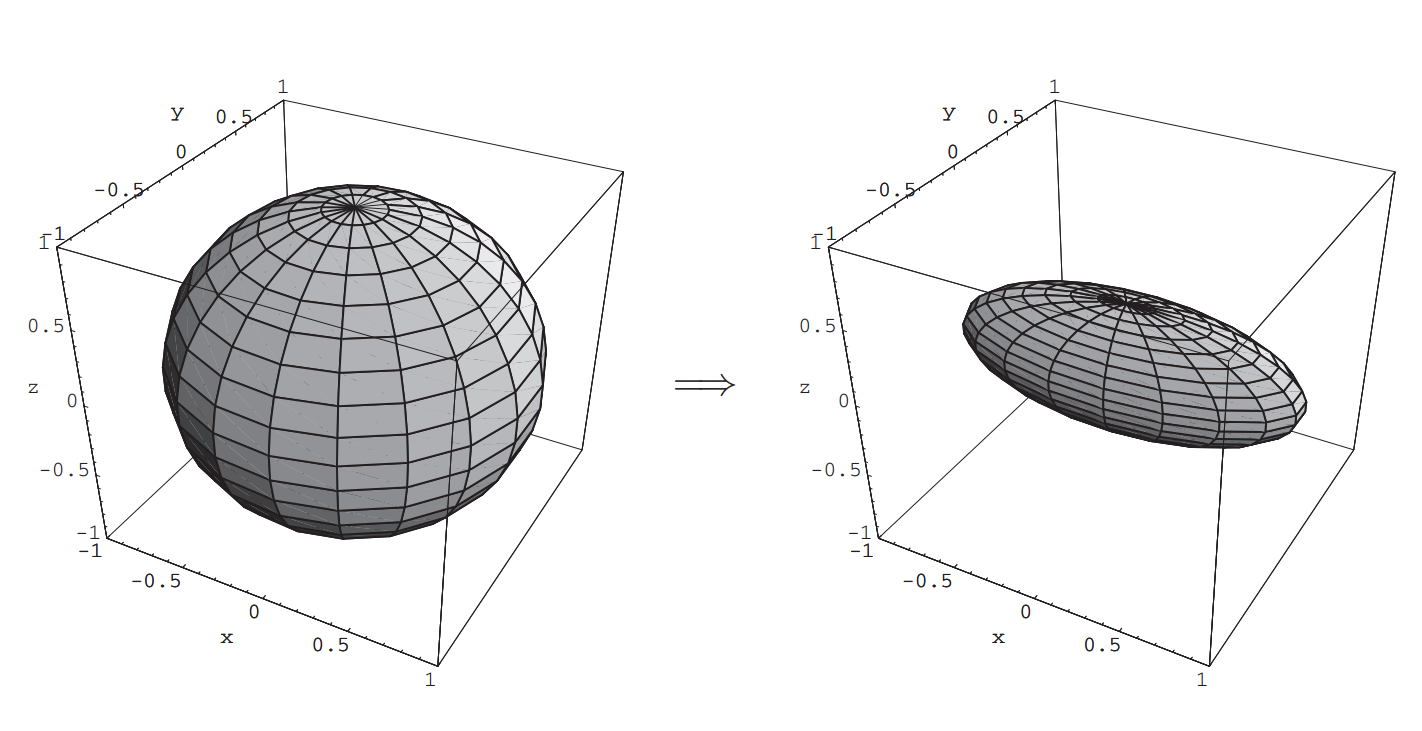
\includegraphics[scale=0.39]{figures/bit_flip.png}
  \centering
  \caption{Effects of a bit flip channel on the Bloch sphere. Taken from~\cite{nielsen_quantum_2010}.}
~\label{fig:bit_flip}
\end{figure} \

\paragraph{Phase Flip} \

A phase flip is defined by the Kraus operators detailed in Equation
~\ref{eq:phase_kraus}. These operators signify that a phase flip
may occur on the quantum state with a probability of \(p\), whereas
the state will remain unchanged with a probability of \(1-p\). If
\(p=1\) then the operation will essentially apply a Z gate. \

\begin{equation}\label{eq:phase_kraus}
  K_0 = \sqrt{1-p} \begin{pmatrix}
          1 & 0 \\
          0 & 1 \\
        \end{pmatrix} \qquad \qquad
  K_1 = \sqrt{p} \begin{pmatrix}
          1 & 0 \\
          0 & -1 \\
        \end{pmatrix}
\end{equation} \

Figure~\ref{fig:phase_flip} depicts the impact of the bit flip
channel when \(p=0.3\). We can appreciate that in the modified
Bloch sphere the \(z\)-axis is left untouched while the \(x-y\)
plane is reduced. Thus, the quantum state becomes less pure. \

\begin{figure}[h!]
  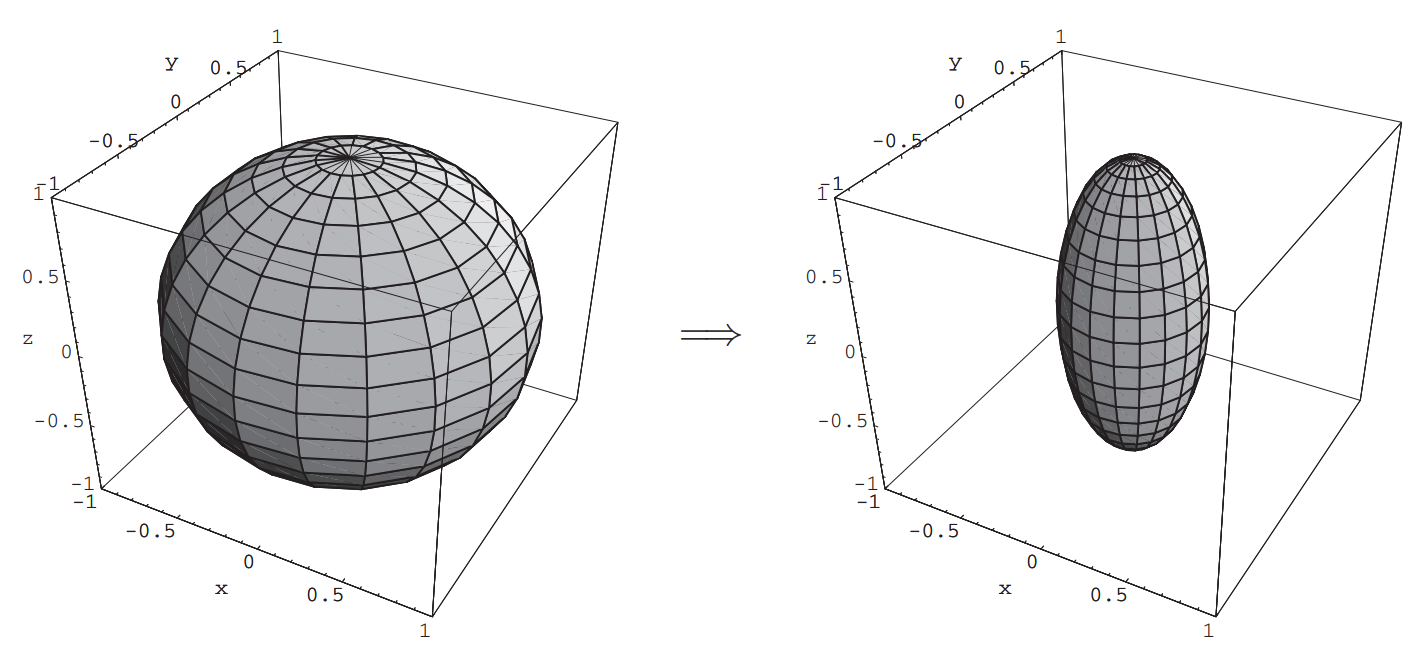
\includegraphics[scale=0.39]{figures/phase_flip.png}
  \centering
  \caption{Effects of a phase flip channel on the Bloch sphere. Taken from~\cite{nielsen_quantum_2010}.}
~\label{fig:phase_flip}
\end{figure} \

\paragraph{Depolarizing Channel} \

The effects that the depolarizing channel has on a quantum state
are described by the Kraus operators in Equation
~\ref{eq:depolarizing_kraus}. The operators describe that with
probability \(p/3\) each of the operators \(X\), \(Y\), and \(Z\)
will be performed. Therefore, the quantum state is not modified with
probability \(1-p\). We can further define the effect of these operators
as \textit{depolarizing} the quantum state with probability \(p\).
Depolarizing a quantum state means substituting \(\rho\) for the maximally
mixed state. \

\begin{equation}\label{eq:depolarizing_kraus}
  \begin{split}
    K_0 = \sqrt{1-p} \begin{pmatrix}
            1 & 0 \\
            0 & 1 \\
          \end{pmatrix} \qquad \qquad
    K_1 = \sqrt{p/3} \begin{pmatrix}
            0 & 1 \\
            1 & 0 \\
          \end{pmatrix} \\
    K_2 = \sqrt{p/3} \begin{pmatrix}
            0 & -i \\
            i & 0 \\
          \end{pmatrix}  \qquad \quad
    K_3 = \sqrt{p/3} \begin{pmatrix}
            1 & 0 \\
            0 & -1 \\
          \end{pmatrix}
  \end{split}
\end{equation} \

In Figure~\ref{fig:depolarizing_flip}, we observe the effects of the 
depolarizing channel with a probability of \(p=0.5\). Notably, the
magnitude shrinks evenly in the modified Bloch sphere. Consequently,
the quantum state experiences a decrease range from all axis. \

\begin{figure}[h!]
  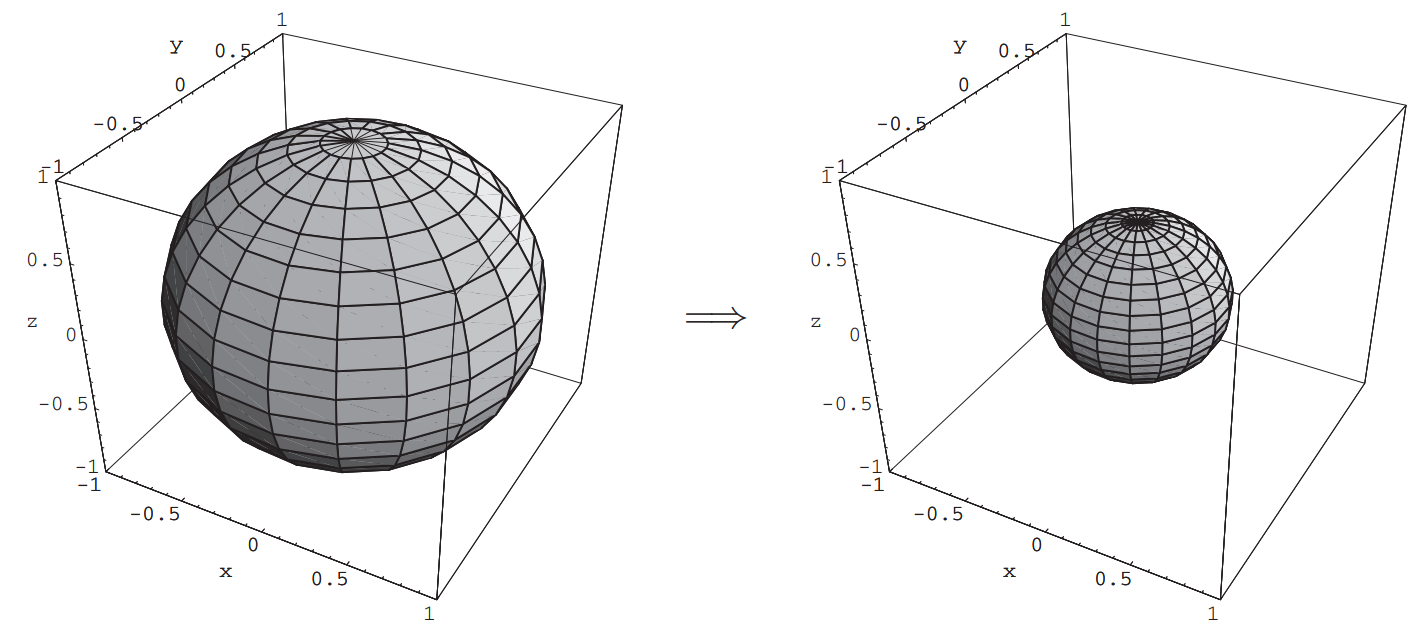
\includegraphics[scale=0.39]{figures/depolarizing_channel.png}
  \centering
  \caption{Effects of a depolarizing channel on the Bloch sphere. Taken from~\cite{nielsen_quantum_2010}.}
~\label{fig:depolarizing_flip}
\end{figure} \

\paragraph{Amplitude Damping} \

The effects of amplitude damping can be equated to
\textit{energy dissipation} in the quantum system. Interaction with
the environment might lead to physycal phenomena like scattering,
dissipation, attenuation, and spontaneous emission, which are all
described by the effects of amplitude damping. An amplitude
damping channel is defined by the Kraus operators outlined in
Equation~\ref{eq:amplitude_kraus}. The \(K_0\) operator leaves
\(\ket{0}\) unchanged but reduces the amplitude of \(\ket{1}\).
This occurs because there was no loss of energy to the environment,
leading the environment to believe the system is probably in \(\ket{0}\)
rather than \(\ket{1}\). The \(K_1\) operator performs a a bit
flip to \(\ket{1}\) and reduces its amplitude by a factor of
\(\sqrt{\gamma}\), where \(\gamma\) is the damping strength.
This operation signifys that the state lost energy to the
environment. \

\begin{equation}\label{eq:amplitude_kraus}
  K_0 = \begin{pmatrix}
          1 & 0 \\
          0 & \sqrt{1-\gamma} \\
        \end{pmatrix} \qquad \qquad
  K_1 = \begin{pmatrix}
          0 & \sqrt{\gamma} \\
          0 & 0 \\
        \end{pmatrix}
\end{equation} \

Figure~\ref{fig:amplitude_damping} illustrates the impact of the
amplitude damping channel with a probability of \(p=0.8\). Remarkably,
the magnitude contracts across the modified Bloch sphere and is pulled
towards the \(\ket{0}\) pole. As a result, the quantum state undergoes
a reduction in possible quantum states values. \

\begin{figure}[h!]
  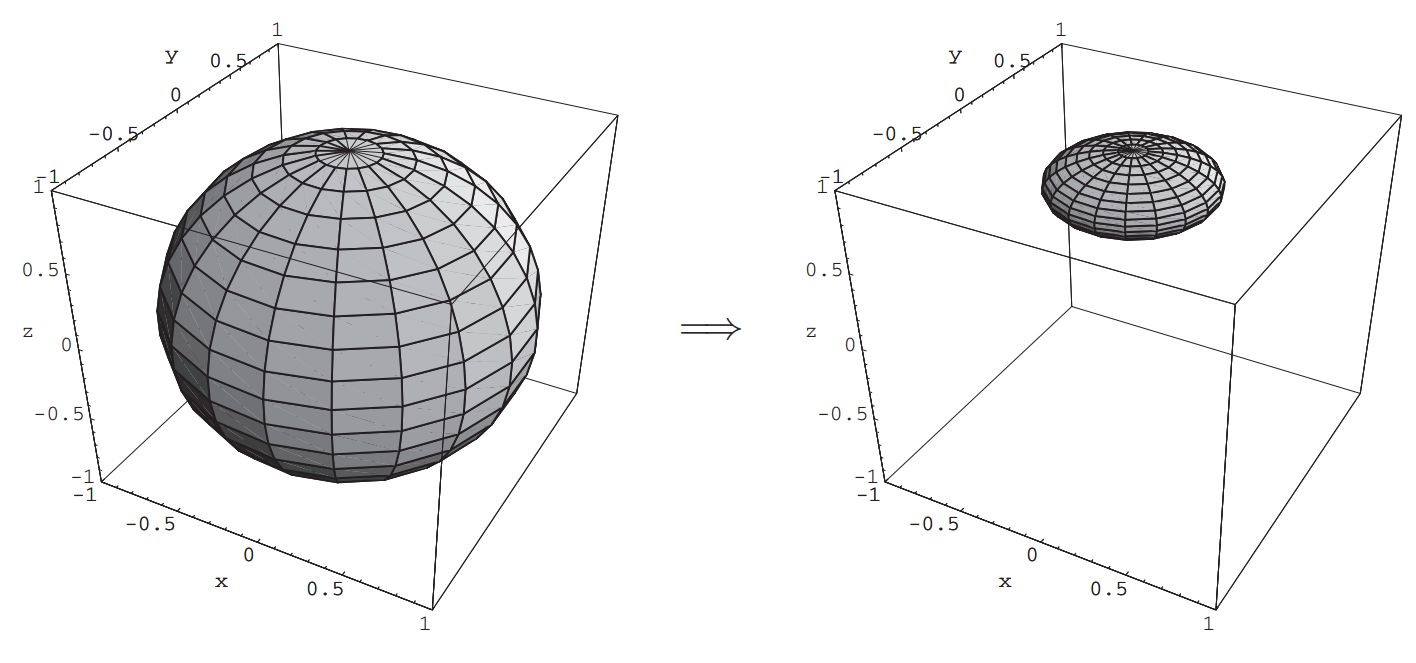
\includegraphics[scale=0.39]{figures/amplitude_damping.png}
  \centering
  \caption{Effects of an amplitude damping channel on the Bloch sphere. Taken from~\cite{nielsen_quantum_2010}.}
~\label{fig:amplitude_damping}
\end{figure} \

\paragraph{Phase Damping} \

The effects of phase damping are unique to quantum mechanics, where
a loss of information occurs without losing any energy. A phase
damping channel is characterized by the Kraus operators presented
in Equation~\ref{eq:phase_damping_kraus}. Similar to amplitude
damping's \(K_0\), \(\ket{0}\) remains unchanged and the amplitude
of \(\ket{1}\) is reduced. However, \(K_1\) consumes \(\ket{0}\)
and reduces the amplitude of \(\ket{1}\). \

\begin{equation}\label{eq:phase_damping_kraus}
  K_0 = \begin{pmatrix}
          1 & 0 \\
          0 & \sqrt{1-\gamma} \\
        \end{pmatrix} \qquad \qquad
  K_1 = \begin{pmatrix}
          0 & 0 \\
          0 & \sqrt{\gamma} \\
        \end{pmatrix}
\end{equation} \

To better understand the effects of phase damping, we can derive equivalent but
differently expressed Kraus operators. In Equation~\ref{eq:phase_damping_kraus_mod}
with \(\alpha = \left(1 + \sqrt{1 - \lambda}\right)\) we can rewrite the
Kraus operators such that they correspond to the phase flip's operators with
the probabilities inversed. This is important because while the physical
quantum process don't match, the transformation of the quantum state due to
the noise is the same. Thus, the effect of phase damping on the Bloch sphere
can be observed in Figure~\ref{fig:phase_flip}. \

\begin{equation}\label{eq:phase_damping_kraus_mod}
  K'_0 = \sqrt{\alpha} \begin{pmatrix}
    1 & 0 \\
    0 & 1 \\
  \end{pmatrix} \qquad \qquad
  K'_1 = \sqrt{1-\alpha} \begin{pmatrix}
    1 & 0 \\
    0 & -1 \\
  \end{pmatrix}
\end{equation} \

% MAYBE: add fidelity, infidelity, diamond distance measure (iverson and preskill)
% MAYBE: state correlation (pravia)

\section{Quantum Machine Learning} \

% TODO: Introduce the subsections from the chapter and link them.

% TODO: Present the difference between QML and classical ML. ~\cite{biamonte}

% TODO: Present encoding dilemma and amplitude encoding.

i.	Introduce variational quantum circuits. \

% TODO: Introduce VQA's / ~\cite{cerezo}

ii.	Explain quantum kernel methods. \
% https://pennylane.ai/qml/demos/tutorial_classical_kernels/
% https://pennylane.ai/qml/demos/tutorial_kernels_module/#training-qeks
% TODO: Say what classical kernel methods are / ~\cite{wang}
% TODO: Say what  quantum kernel embeddings are and how to train them / ~\cite{hubregsten}

\section{Adversarial Machine Learning} \

% TODO: Introduce the subsections from the chapter and link them.

i.	State generalization problems.  \

ii.	Present different attacks such as FGSM, C\&W, and PGD\@. \

iii.	Introduce adversarial training as defence mechanism against adversarial attacks. \

iv.	Explain the relationship between general accuracy and adversarial resilience. \